\section{KeyGraph Importacne}
We use KeyGraph Algorithm to improve the effectiveness and quality of our experiment, as we know if we use KeyGraph Algorithm to extract keywords, and disregards others, some information will be lost. It is very necessary to verify that after the processing of KeyGraph Algorithm, the result is still complete and powerful.\\
In this experiment to verify KeyGraph, we use some precedents downloaded from D1.com to see how KeyGraph will influence the connections between events. Whether the quality of events is influenced by disregarding some nouns.\\ \\
\textbf{Experiment}\\ \\
\begin{table}[!h]
\centering
\begin{tabular}{ccc}
\hline
Serial number&Precedent ID&Precedent Name\\
068&28110821&\begin{CJK}{UTF8}{ipxm}損害賠償請求事件-中国残留孤児国賠訴訟\end{CJK}\\
069&28111682&\begin{CJK}{UTF8}{ipxm}損害賠償請求事件-損害賠償等請求事件\end{CJK}\\
085&28162030&\begin{CJK}{UTF8}{ipxm}損害賠償請求事件-独立当事者参加事件\end{CJK}\\
\hline
\end{tabular}
\end{table}
\\ \\
Using all KNP results of each document, find all of the events, and check the proportion of events connected by high KeyScore nouns.\\ \\ 
\textbf{Result}\\ \\
\begin{figure}[!h]
\centering
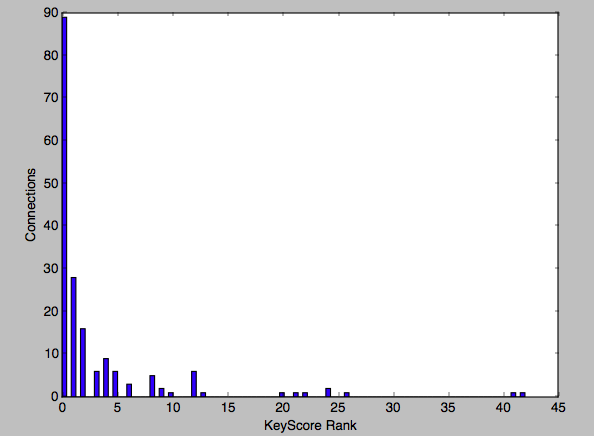
\includegraphics[width=300pt]{./pictures/0402-0.png}
\caption{Result of Experiment}
\end{figure}
The figure only shows top-45 rank KeyScore nouns because, after that, the connections between nouns are very less. And we can also find that main connections are between High KeyScore nouns, special top-25 ones. So in our experiment, we choose top-25 KeyScore nouns will be a very safe and efficient way.